\subsection{Pedido de ventas con transporte propio}

%!!! cambiar esto por el diagrama de visio cuando este :)
\subsubsection{Cursograma}
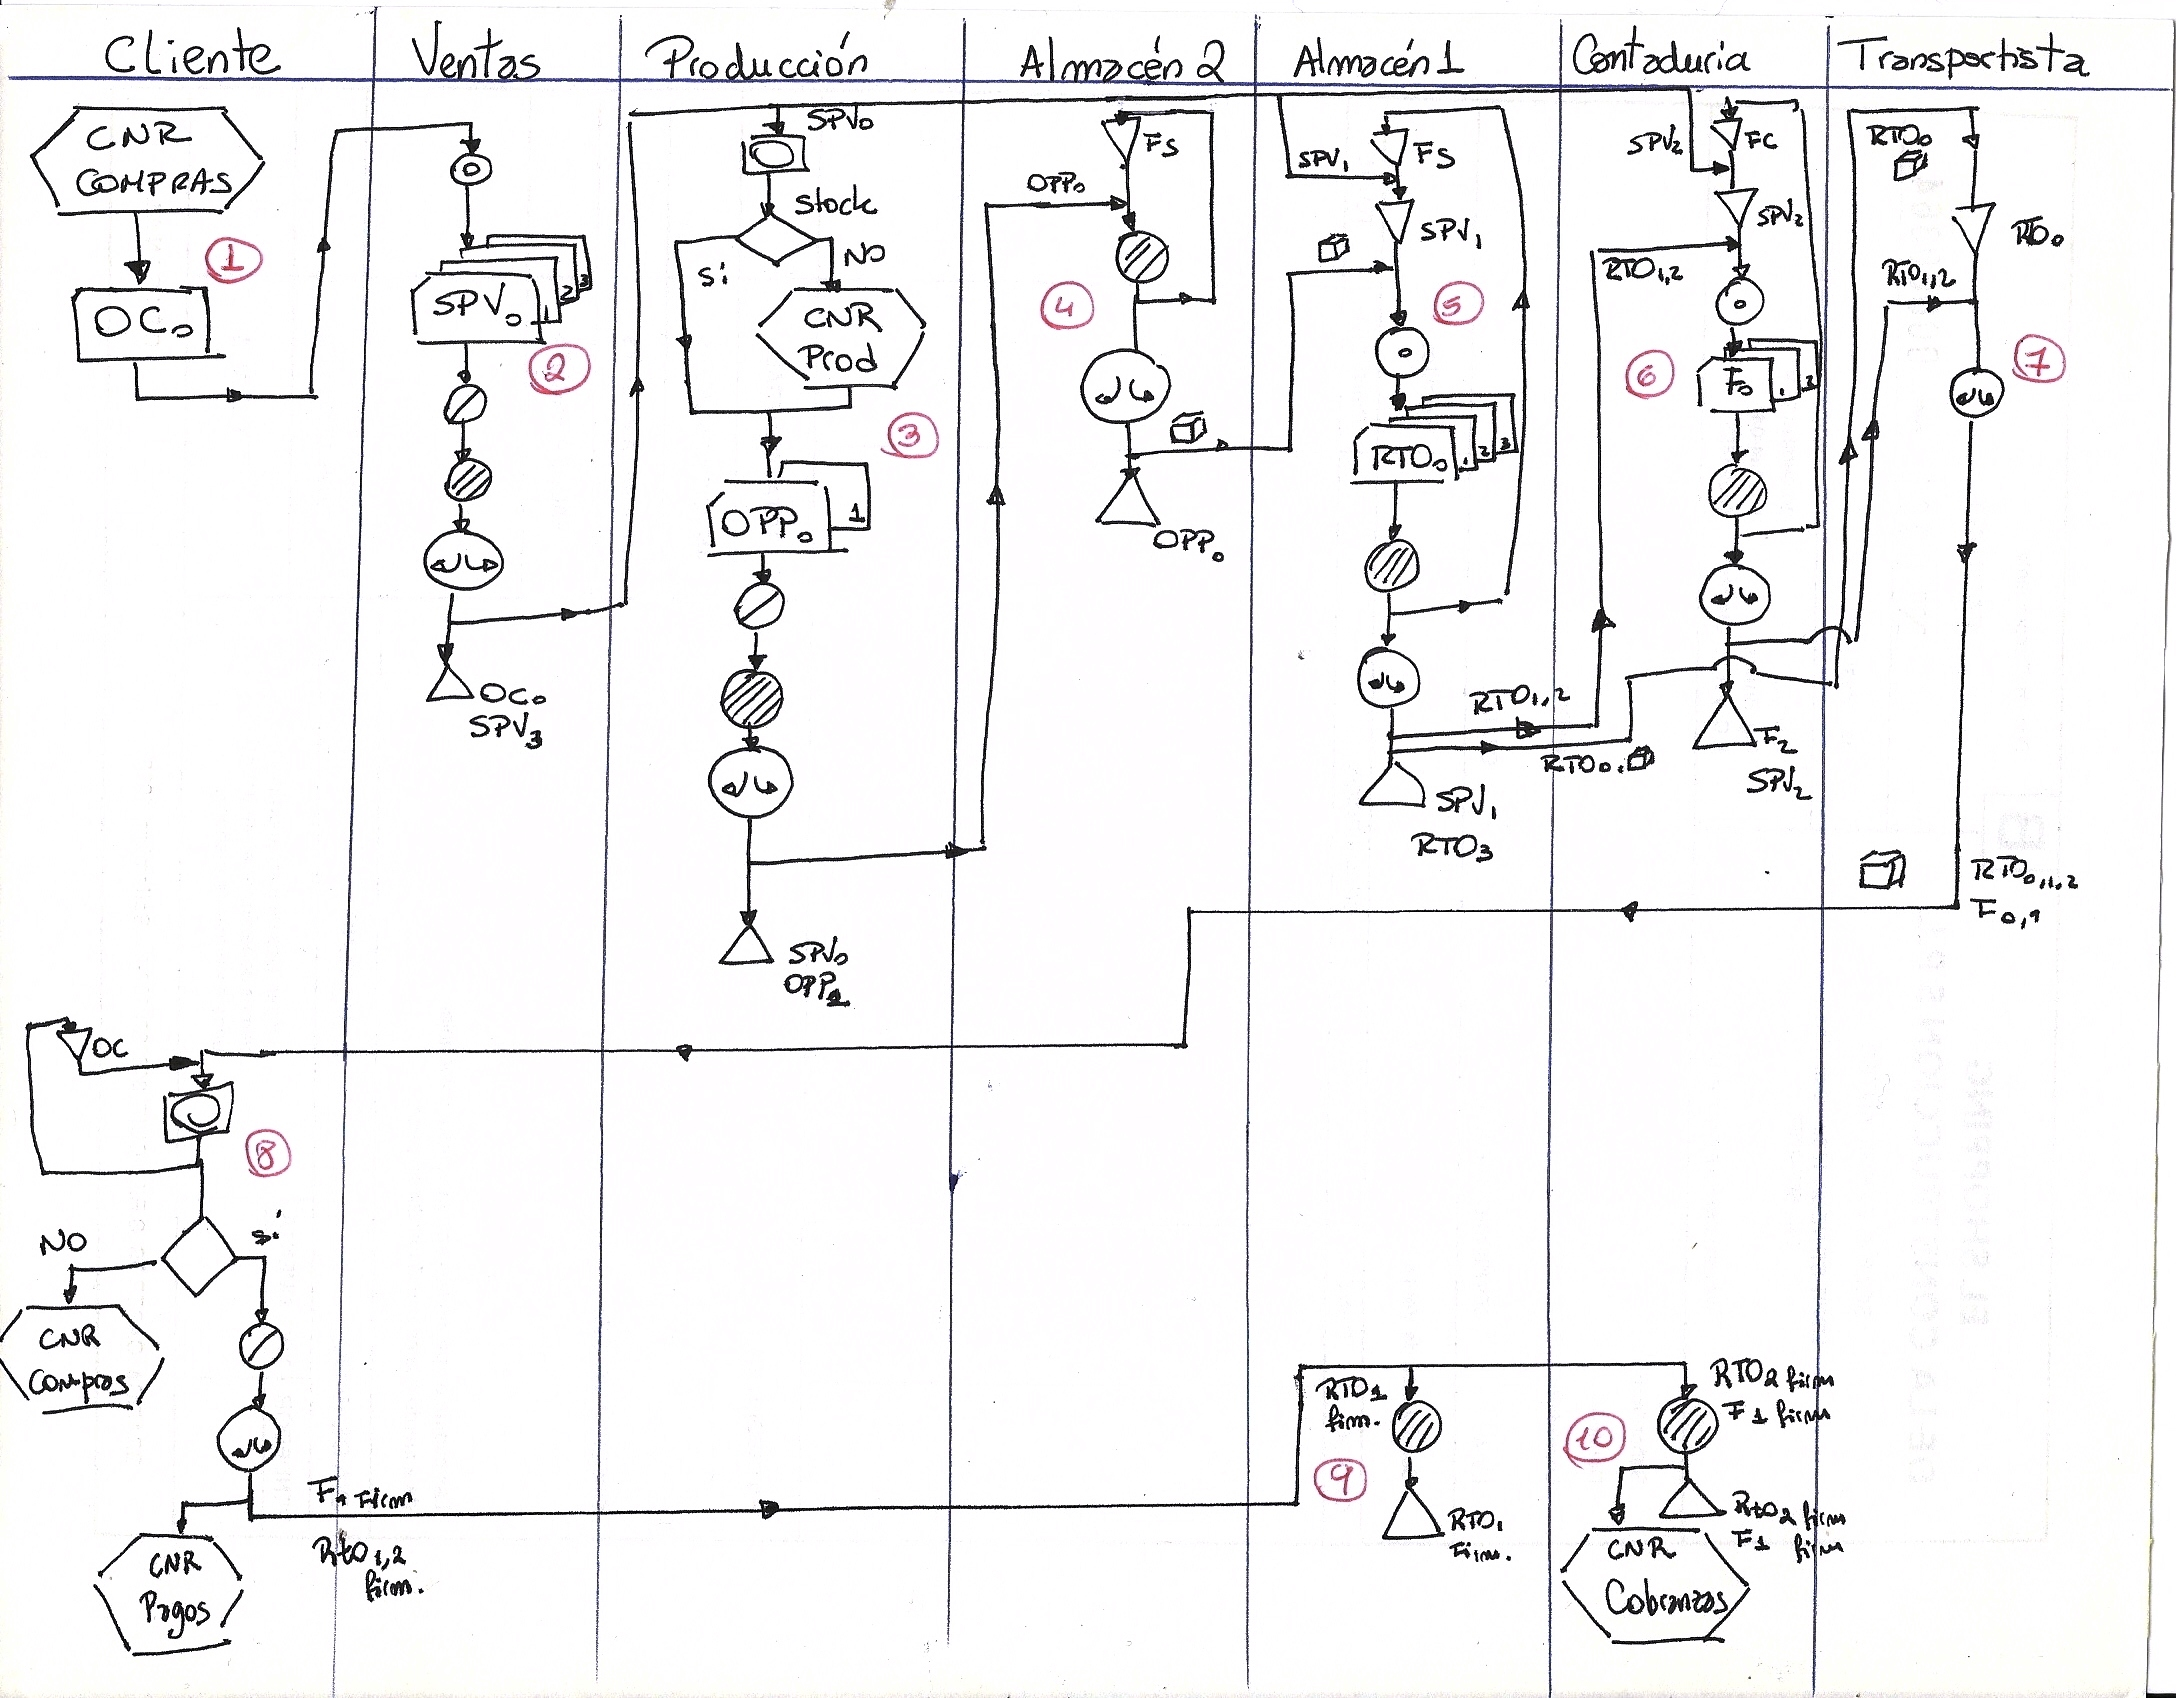
\includegraphics [angle=90]{Empresa/Circuitos/Ventas/ventas.jpg}

\pagebreak

\subsubsection{Procedimiento}
\begin{enumerate}
\item El cliente solicita un pedido
\item Ventas genera la Solicitud de Pedido de Ventas (SPV) especificando los detalles de la venta (productos, plazo de entrega tentativo).
	Firma la SPV y envia una copia a Producci\'on. Archiva temporalmente esta solicitud hasta que concluya el pedido.
\item Producci\'on recibe la SPV y verifica que cuenta con stock. De no poseer stock necesario se procede a realizar el CNR de Producci\'on. 
	En caso de contar con el producto solicitado, se envia ``una orden de pedido de productos'' a Almac\'en 2 ( almacén de productos terminados ).
\item Almac\'en 2 recibe la orden de producto ( ya cuenta con el producto, ya sea porque ten\'ia stock o porque lo ha producido especialmente ) y lo env\'ia al  Almac\'en 1 ( Expedici\'on).
\item Almac\'en 1 prepara los productos para su entrega y genera el remito correspondiente, con 2 copias. Entrega el producto al Transportista con los remitos original y copia para que sean firmados por el cliente y env\'ia otra copia a Contadur\'ia.
\item Contadur\'ia genera un listado de remitos sin facturar asociados a esa SPV, y genera la factura correspondiente. Se envia el original de la factura al Transportista para su env\'io.
\item Transportista recibe original y copia del remito y la factura. Env\'ia el pedido junto con la documentaci\'on al cliente.El cliente recibe el original de la factura y del remito, y firma la copia del remito.
\item Almacen 1 recibe la copia del remito firmado por el cliente y cierra la orden de pedido. 
\item Contadur\'ia recibe la copia de la factura y el remito firmado por el cliente y la asienta como recibida por el cliente. El pago de la factura es parte del CNR de Cobros.Contaduria
\end{enumerate}

